\chapter{场景建模}
    
    \section{Web API}
        Web API是网络服务对外提供的接口, 当前, 以RESTful风格API的使用最为普遍, 本文的web API场景建模与自动化测试亦主要针对RESTful风格的web API.
        
        这类web API虽然根据具体的web服务而各不相同, 甚至差异巨大, 但由于大致遵从REST风格\cite{fielding2000architectural}, 也拥有许多共同点:
        
        \begin{itemize}
            \item API使用HTTP网络协议, 部分亦使用HTTPS协议. 基于客户端 - 服务器的交互方式, 即"请求 - 响应"模式, 且拥有无连接, 无状态的特征.  
            
            \item 使用URI(统一资源标识符)指明所需资源, 通常使用URL的形式.
            
            \item 数据传输时通常使用简明的数据表示协议, 如JSON, XML, HTML等.
        \end{itemize}
        
        一个web API的请求通常包含以下要素:
        \begin{itemize}
            \item 请求协议: 如HTTP, HTTPS等, 包含签名机制的API, 其签名协议亦可考虑在内.
            
            \item URL: 请求的路径, 也包括主机地址/域名.
            
            \item 请求方法: 请求的方法, 结合请求路径, 通常反映了API的大致含义, 如\texttt{GET}, \texttt{POST}等.
            
            \item 请求头: 请求头是键值对的列表, 其中包括\texttt{content-length}等常见域, 也常有API的定制域和签名域, 用于向服务器发送关键信息.
            
            \item 请求体: 请求体是可选的, 通常用于向服务器传送体量较大的数据对象, 除了常见的JSON和XML等数据格式外, 也可以是二进制文件或媒体文件.
        \end{itemize}
        
        一个web API的响应则通常由以下部分组成:
        \begin{itemize}
            \item 响应状态码: web API的响应状态码, 通常为3位数字, 且有约定的语义含义. 如2XX表示请求成功, 4XX表示资源不存在, 5XX表示服务器内部错误.
            
            \item 响应头: 类似于请求头, 也是键值对的列表, 服务器常通过定制域向客户发送关键信息.
            
            \item 响应体: 类似请求体, 响应体也是可选的, 通常用于服务器返回体量较大的资源或数据对象. 如HTML网页, JSON或XML数据对象, 文件等等.
        \end{itemize}
        
        如\ref{sec:research_status}小节所述, OpenAPI\cite{openapi17}是一种专门描述RESTful web API行为的规约语言, 它基于YAML格式, 提供了详细的格式定义, 用一种形式化, 规范化的形式描述web API的包括但不限于以上所介绍的各请求要素. 此外, 对于请求/响应的头/体, 若值数据为较简单的数据对象如JSON和XML对象, OpenAPI还可以递归描述其各个成员或各个元素的类型, 取值区间等详细信息, 以及序列化方式(如空格分隔, 分号分隔等), 相当于定义了它们的合法取值集合.
        
        \begin{figure}[!htb]
            \centering
            \scriptsize
            \tt
            
                \begin{lstlisting}[language=yaml]
openapi: 3.0.0
servers: [url: 'oss://127.0.0.1:8080']
info:
  description: Object Storage Service
  version: "1.0.0"
  title: OSS API Series
tags:
  - name: service
    description: Service related operations
components:
  schemas:
    location:
      type: string
      enum: ['oss-cn-beijing']
    error_response:
      type: object
      properties:
        Code: {type: string}
        Message: {type: string}
        RequestId: {type: string}
        HostId: {type: string}
  responses:
    error:
      description: 'error'
      content: {main: {schema: {$ref: '#/components/schemas/error_response'}}}
  parameters: {}
paths:
  /GetService:
    get:
      tags: ['service']
      summary: Return all buckets of current account
      x-realPath: '/'
      operationId: GetService
      responses:
        '200':
          description: 'Success'
          content:
            main:
              schema:
                type: object
                xml: {name: ListAllMyBucketsResult}
                properties:
                  Owner:
                    type: object
                    properties:
                      ID: {type: string}
                      DisplayName: {type: string}
                  Buckets:
                    type: array
                    xml: {wrapped: true}
                    items:
                      type: object
                      xml: {name: Bucket}
                      properties:
                        Name: {type: string}
                        CreateDate: {type: string, format: date-time}
                        Location: {$ref: '#/components/schemas/location'}
                        ExtranetEndpoint: {type: string}
                        IntranetEndpoint: {type: string}
                        StorageClass: {type: string}
        default: {$ref: '#/components/responses/error'}
                \end{lstlisting}
            
            \caption{OpenAPI脚本示例. 该脚本定义了对象存储服务的一个名为\texttt{GetService}的API. 此API无请求参数, 响应体根据响应状态码的不同而有不同格式, 分为200和异常状态码两种情形, 响应体亦定义了数据对象与其XML表示的对应关系.}
            \label{fig:openapi_example}
        \end{figure}
        
        如图\ref{fig:openapi_example}为一段OpenAPI脚本示例, 这段脚本在后文的实验部分被直接用到, 它定义了名为\texttt{GetService}的web API.
        
        一个web服务通常由一系列API组成, 在web服务的描述中, 一个API对应着服务的一项具体功能, 也是服务的一个具体接口, 因此对应着一个服务端点. 在进行场景建模时, 本文对服务端点/API的形式化模型进行了适当抽象, 视为一个由\textbf{API名称}, \textbf{合法请求数据}(包括请求体与请求头键值对列表)集合和\textbf{合法响应数据}(包括响应体, 响应头列表和响应状态码)集合构成的三元组. 对于请求协议, URL等与使用场景描述相关度较小的要素则视为API名称的一部分.
    
    \section{概率有限状态自动机}
        
        概率有限状态自动机(PFSA)是非确定性有限状态自动机(NFA)的扩展. 它将概率因素引入非确定性有限状态自动机的转移, 起始状态和终止状态中.
        
        根据Enrique Vidal等人的阐述\cite{enriquev05}, 基本的概率有限状态自动机具有如下的定义(定义\ref{def.pfsa}).
        
        \begin{definition}
            \label{def.pfsa}
            概率有限状态自动机为一个元组
            \begin{equation}
                \mathcal{B} := <Q_{\mathcal{B}}, \Sigma, \sigma_{\mathcal{B}}, I_{\mathcal{B}}, F_{\mathcal{B}}, P_{\mathcal{B}}>,
            \end{equation}
            
            其中:
            \begin{itemize}
                \item $Q_{\mathcal{B}}$是有限的状态集合;
                
                \item $\Sigma$是字符集;
                
                \item $\sigma_{\mathcal{B}} \subseteq Q_{\mathcal{B}} \times \Sigma \times Q_{\mathcal{B}}$是状态转移的集合;
                
                \item $I_{\mathcal{B}} : Q_{\mathcal{B}} \to \mathbb{R}^{+}$是各个状态作为起始状态的概率分布;
                
                \item $F_{\mathcal{B}}: Q_{\mathcal{B}} \to \mathbb{R}^{+}$是于各个状态处终止的概率分布;
                
                \item $P_{\mathcal{B}} : \sigma_{\mathcal{B}} \to \mathbb{R}^{+}$是各条转移边的转移概率.
            \end{itemize}
            
            $I_{\mathcal{B}}$函数满足初始状态概率归一化性质:
            \begin{equation}
                \label{eq:pfsa_init_normal}
                \sum_{q \in Q_{\mathcal{B}}} I_{\mathcal{B}}(q) = 1.
            \end{equation}
            
            $F_{\mathcal{B}}$和$P_{\mathcal{B}}$函数满足转移概率归一化性质:
            \begin{equation}
                \label{eq:pfsa_trans_normal}
                \forall q \in Q_{\mathcal{B}}, \forall a \in \Sigma, F_{\mathcal{B}}(q) + \sum_{q' \in Q_{\mathcal{B}}, (q,a,q') \in \sigma_{\mathcal{B}}} P_{\mathcal{B}}(q,a,q') = 1.
            \end{equation}
        \end{definition}
        
        在定义中, 基本的组成单位为"状态", 状态集合$Q_{\mathcal{B}}$与之对应. 字符集则由$\Sigma$定义. 状态之间由转移边连接起来, 转移边除了连接两个状态之外, 还有两个重要元素: 字符与转移概率, 其中字符为字符集的元素, 而转移概率为非零实数. 状态转移的集合由$\sigma_{\mathcal{B}} \subseteq Q_{\mathcal{B}} \times \Sigma \times Q_{\mathcal{B}}$定义, 它指明了连接的两个状态和字符, 而转移概率则由函数$P_{\mathcal{B}} : \sigma_{\mathcal{B}} \to \mathbb{R}^{+}$定义. 起始状态则由$I_{\mathcal{B}} : Q_{\mathcal{B}} \to \mathbb{R}^{+}$定义, 这是一个定义在状态集合上的函数, 它描述了每个状态作为初始状态的概率. 这与确定有限状态自动机(DFA)中初始状态的定义为某一固定状态$q_0 \in Q$不同. 终止的定义则为$F_{\mathcal{B}}: Q_{\mathcal{B}} \to \mathbb{R}^{+}$, 这个状态集合上的函数定义了在每个状态上终止的概率.
        
        由于$I_\mathcal{B}, F_\mathcal{B}, P_\mathcal{B}$均描述概率, 故它们满足一定的归一化性质. 其中, 式\ref{eq:pfsa_init_normal}表示所有状态成为初始状态的概率为1, 这保证了自动机工作时一定能随机确定一个初始状态. 式\ref{eq:pfsa_trans_normal}表示当自动机处于任意状态时, 对于任意字符, 其终止的概率加上所有可用的转移的概率之和为1, 这保证了自动机在每一步都能随机性地确定是否终止或进行某项转移.
        
        对于一个输入串$S \in \Sigma^{*}$, 概率有限状态自动机的工作方式分为两步:
        \begin{enumerate}
            \item 初始化: 按照概率分布$I_\mathcal{B}$选择一个$Q_{\mathcal{B}}$中的状态$q_0$作为初始状态;
            
            \item 生成: 每一步依次读入一个$S$中的字符, 设当前读入的字符为$a, a \in \Sigma$, 当前状态为$q$. 则以$F_{\mathcal{B}}(q)$的概率决定是否在此状态处终止, 或者, 对$\forall (q, a, q') \in \sigma_{\mathcal{B}}$, 以$P_{\mathcal{B}}(q, a, q')$的概率决定是否进行转移$(q,a,q')$. 如果进行此转移, 则将$q'$置为当前状态.
        \end{enumerate}
        当读入串$S$的\textbf{过程中}或读入\textbf{结束后}, 若自动机终止, 则当前串$S$被定义为可被自动机\textbf{接受}.
        
        由以上步骤可以看出, 概率有限状态自动机是一种随机模型, 它定义了每个串$S \in \Sigma^{*}$是否被自动机$\mathcal{B}$接受的概率, 它生成的是有限串集合$\Sigma^{*}$上的概率空间, 即概率分布函数.
        
        \begin{figure}[!htb]
            \centering
            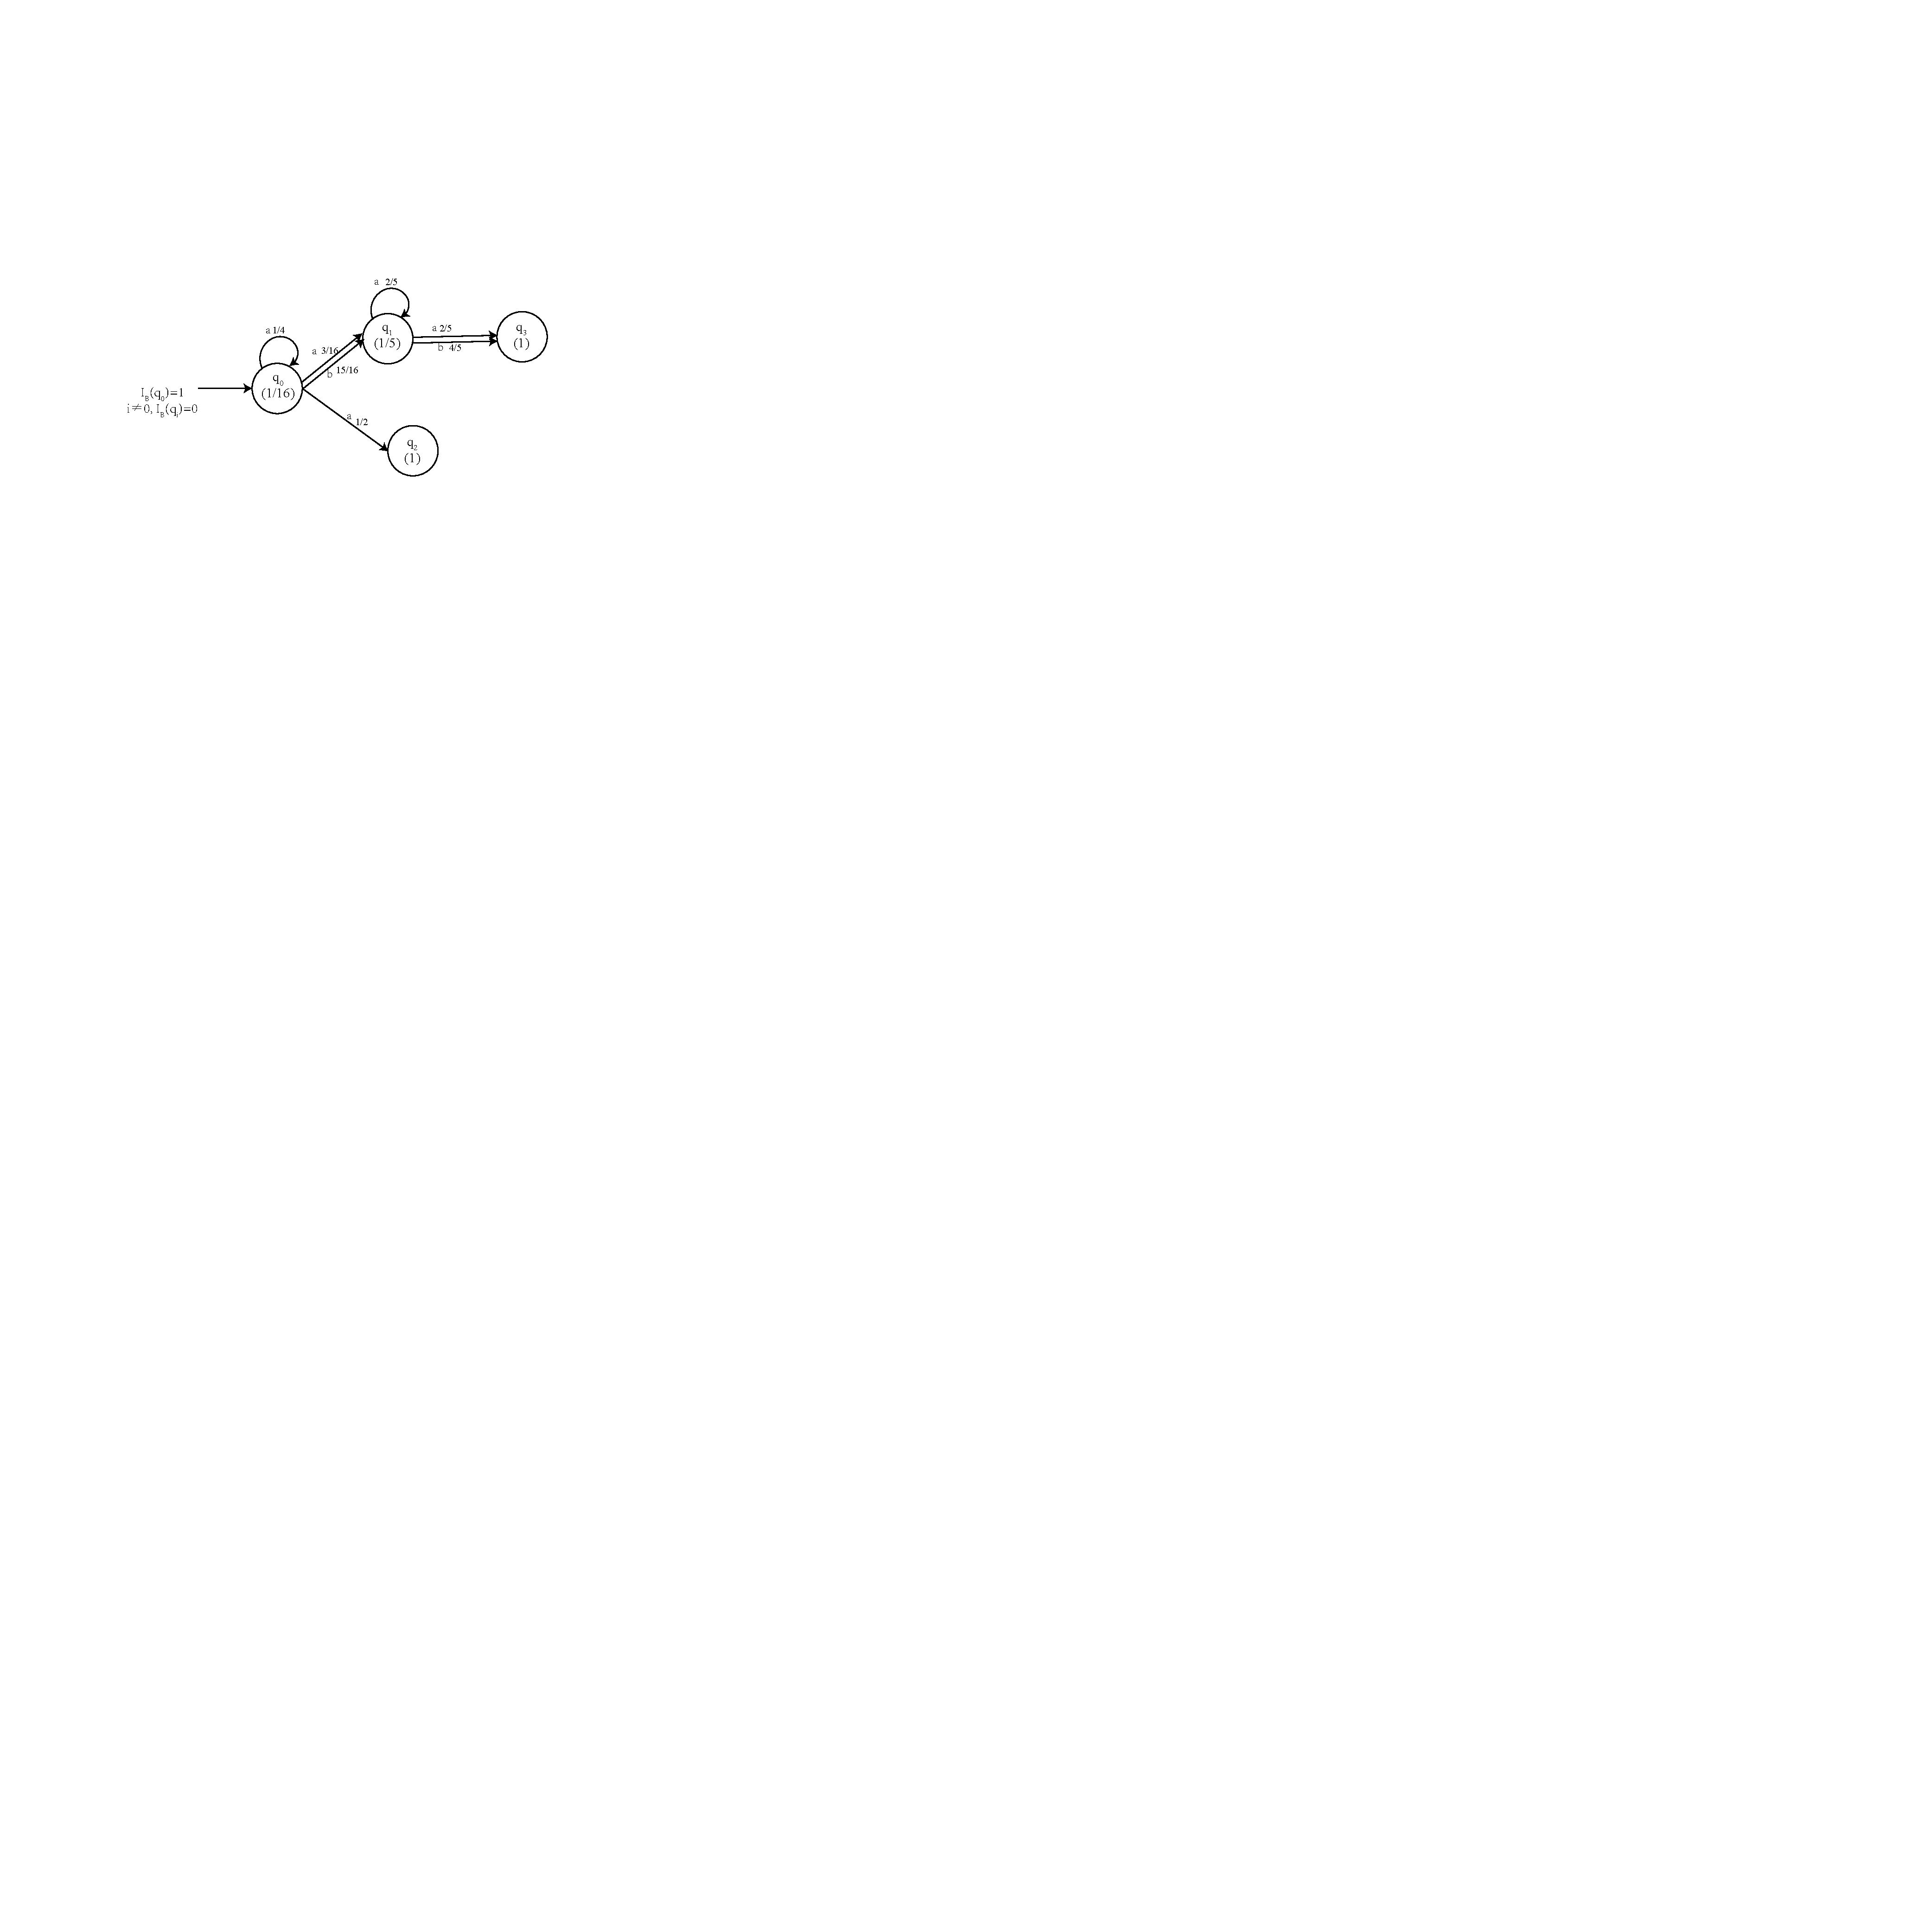
\includegraphics[width=400pt]{PFSA_example.pdf}
            \caption{概率有限状态自动机示例. 以有向图的形式可视化表示.}
            \label{fig:PFSA_example}
        \end{figure}
        
        类似于确定性有限状态自动机, 概率有限状态自动机也常常使用带标签边的有向图表示. 图\ref{fig:PFSA_example}展示了一个概率有限状态自动机的例子. 其中, 图的节点表示自动机的状态, 图的带标签边表示自动机的概率转移边, 图中节点上的数字表示自动机状态的终止概率. 图中所示的概率有限状态自动机共有4个状态, $I_{\mathcal{B}}(q_0)=1; I_{\mathcal{B}}(q_i) = 0, i \neq 0$表示该自动机的初始状态仅有$q_0$, 为确定性的. 终止方面, $q_0$的终止概率为$1/16$, $q_1$的终止概率为$1/5$, $q_2$和$q_3$的终止概率均为1. 可以很方便地计算出图中示例对于某一字符串的接受概率, 如$P_{accept}("aa") = 84.4\%, P_{accept}("ab") = 81.3\%$.
        
    \section{建模需求}
        \textbf{使用场景模型}是一种有效的模型化技术. 使用场景模型可以描述在现实世界中, 一或多个人如何与系统进行交互\footnote{http://agilemodeling.com/artifacts/usageScenario.htm}. 模型表达了交互过程中的步骤, 事件和动作. 本文提出了一种web API的使用场景模型, 该模型的设计目标与需求为: 1)为web API的复杂组合测试的自动化生成提供基础; 2)为丰富多样的实际用户使用场景提供描述能力; 3)具有足够的抽象程度便于分析与对比.
        
        经过大量API分析调研与实践, 本文总结出模型应描述web API的以下特性:
        \begin{itemize}
            \item 与使用场景相关的服务端点元素. \\
            这包括服务端点的协议, 路径, 合法请求体格式, 合法响应体格式等.
            
            \item 用户使用时的API请求调用序列. \\ 由于一个典型的web服务由一系列API组成, 使用此web服务总涉及到对多个API的先后调用, 因此调用序列的表达不可或缺. 这包括API对之间的先后顺序, 如"注册用户"应在"登录"之前执行, "注销"应在"登录"之后执行等等; 也包括频繁连续调用序列的表达.
            
            \item API调用序列的数据传递与依赖. \\
            在一次会话的API调用序列中, 之前调用的API的请求数据/响应数据常常与之后调用的API的请求数据/响应数据有关联和依赖. 如之前调用"登录"API时获得的用户ID信息, 在之后调用"浏览"或"上传"等具体功能API时需用来填充用户ID这一参数.
            
            \item API调用序列的条件与分支. \\
            实际使用场景中, 用户常根据返回的状态与信息选择不同的操作, 因此需要在场景模型中引入与实际响应数据相关的条件与判断, 并允许根据判断结果执行不同后继序列.
            
            \item 测试断言. \\
            为满足场景的测试目标, 需要在场景模型中引入参照, 这里的参照即为断言, 断言既包括数据流断言也包括控制流断言.
            
            \item 不同API请求的频率.\\
            对于一个web服务的各个API服务端点, 用户使用的频率是不等的. 一方面为了描述实际使用, 另一方面需要使频繁使用的API和调用序列被更多地测试, 故需要使场景模型包含不同API的频率信息.
        \end{itemize}
        
        本文提出的场景模型以概率有限状态自动机(PFSA)模型为基础, 这是因为, 概率有限状态自动机有以下特点适于对web API的使用场景进行建模:
        \begin{itemize}
            \item 每个自动机的状态可以关联一个固定的服务端点/API. 每一步对该状态关联的API发送请求进行调用. 那么, 状态序列即可建模服务端点的调用与执行序列. 自动机所有能确定性正常接受的字符串则建模了一个测试用例和一次通过了此测试用例的测试执行.
            
            \item 将每一步中, API调用的响应数据作为当前字符, 则自动机的字符集$\Sigma$可建模一个web服务所有服务端点API的合法响应数据集合. 另一方面, 每个状态转移均对应一个字符$c \in \Sigma$, 其表示此转移仅限当前读入字符为$c$时使用. 因此, 此字符可建模各个转移所适用的范围, 此范围由服务端点API的实际响应数据决定. 也就是状态转移对应的字符定义了进行此状态转移的条件, 同时也引入了分支结构. 不过该条件仅与当前响应数据相关.
            
            \item 自动机的起始概率, 终止概率, 转移概率反映了与各服务端点API进行交互的频率差异.
            
            \item 自动机概率性质的存在, 使得其每次工作时经过的状态与选择的转移都不尽相同, 对应生成的测试用例也就不尽相同. 相比确定性自动机只能生成单一执行序列/测试用例, 概率性自动机可生成多样用例的性质有明显优势.
        \end{itemize}
        
        然而, 对照需求, 概率有限状态自动机仍有其明显的不足之处: 1)不能表达API调用序列的数据传递与依赖. 由于在自动机模型中, 状态本身的定义只是可以与某一API服务端点关联, 故并不能在其上定义请求数据与响应数据的这种数据流关系. 2)数据流测试断言的表达. 测试断言的需求包括控制流断言与数据流断言, 控制流断言即对生成序列进行限制, 这可以通过终止条件或引入表示测试失败的"非法/fail"状态表达. 但是数据流的断言是定义在请求数据与响应数据上的, 故无法表达.

        本文的场景模型扩展了概率有限状态自动机模型来克服这一问题.
    
    \section{场景模型定义}
        相比于最基本的概率有限状态自动机, 本文的场景模型主要对其状态的定义进行了扩展:
        \begin{itemize}
            \item 在状态定义中允许与服务端点名称的关联.\\
            这样便可以与具体API服务端点进行关联, 从而建模API请求调用.
        
            \item 在状态定义中加入了请求数据约束与响应数据约束的定义.\\
            这是对API描述脚本中请求数据与响应数据的格式与求值约束的抽象. API描述的这一部分亦是场景模型中数据流定义的重要组成部分.
            
            \item 在状态定义中加入了请求数据依赖.\\
            此定义描述了当前状态的请求数据与执行序列的所有前驱状态的请求/响应数据的依赖关系.
            
            \item 在状态定义中加入了响应数据断言.\\
            此定义弥补了基本模型不能描述数据流测试断言的缺陷.
        \end{itemize}
        
        场景模型的形式化定义如下:
        
        \begin{definition}
            \label{def:our}
            场景模型是一个元组
            \begin{equation}
                \label{eq:scenario_model}
                 \mathcal{A} := <Q_{\mathcal{A}}, \Sigma, \sigma_{\mathcal{A}}, I_{\mathcal{A}}, F_{\mathcal{A}}, P_{\mathcal{A}}>,
            \end{equation}
            
            其中:
            \begin{itemize}
                \item $Q_{\mathcal{A}}$是有限的状态集合;
                
                \item $\Sigma$是此web服务所有API的合法响应的集合;
                
                \item $\sigma_{\mathcal{A}} \subseteq Q_{\mathcal{A}} \times \Sigma \times Q_{\mathcal{A}}$是状态转移的集合;
                
                \item $I_{\mathcal{A}} : Q_{\mathcal{A}} \to \mathbb{R}^{+}$是各个状态作为起始状态的概率分布;
                
                \item $F_{\mathcal{A}} : Q_{\mathcal{A}} \to \mathbb{R}^{+}$是于各个状态处终止的概率分布;
                
                \item $P_{\mathcal{A}}: \sigma_{\mathcal{A}} \to \mathbb{R}^{+}$是各条转移边的转移概率.
            \end{itemize}
            
            对于$I_{\mathcal{A}}$, $F_{\mathcal{A}}$, $P_{\mathcal{A}}$, 仍然要求满足归一化性质:
            \begin{equation}
                \label{eq:model_normal1}
                \sum_{q \in Q_{\mathcal{A}}} I_{\mathcal{A}}(q) = 1;
            \end{equation}
            与
            \begin{equation}
                \label{eq:model_normal2}
                \forall q \in Q_{\mathcal{A}}, \forall a \in \Sigma, F_{\mathcal{A}}(q) + \sum_{q' \in Q_{\mathcal{A}}, (q,a,q') \in \sigma_{\mathcal{A}}} P_{\mathcal{A}}(q,a,q') = 1.
            \end{equation}
            
            状态$q \in Q_{\mathcal{A}}$的定义是一个元组
            \begin{equation}
                \label{eq:scenario_model_state}
                q := <t_q, in_q, out_q, d_q, a_q>,
            \end{equation}
            其中:
            \begin{itemize}
                \item $t_q$可以为$empty$(表示不与任何API服务端点关联)或某个服务端点的名称;
                
                \item $in_q$是当前状态所有合法请求数据的集合;
                
                \item $out_q$是当前状态所有合法响应数据的集合;
                
                \item $d_q$是请求数据依赖的集合;
                
                \item $a_q$是响应数据断言的集合.
            \end{itemize}
            
            作为所有可能的API响应的集合, $\Sigma$满足
            \begin{equation}
                \Sigma = \bigcup_{q \in Q_{\mathcal{A}}} out_q.
            \end{equation}
            
            在状态$q$的定义中, 每一项请求数据依赖$d \in d_q$都是一个元组
            \begin{equation}
                \label{eq:scenario_request_depen}
                d := <q_d, index_d, f_d>,
            \end{equation}
            它的各项含义为:
            \begin{itemize}
                \item $q_d \subseteq Q_{\mathcal{A}}$是场景模型$\mathcal{A}$中的一个或多个状态的集合;
                
                \item $index_d \in \mathbb{Z}$是一个整数;
                
                \item $f_d: \bigcup_{q' \in q_d} in_{q'} \times out_{q'} \to i \subseteq in_q$是一个函数, 此函数定义了给定状态$q_d$上的请求数据和得到的响应, 对当前状态$q$而言, 合法的请求数据集合.
            \end{itemize}
            
            在状态$q$的定义中, 每一项响应数据的断言$a \in a_q$也是一个元组
            \begin{equation}
                a := <q_a, index_a, f_a>,
            \end{equation}
            它的各项含义为:
            \begin{itemize}
                \item $q_a \subseteq Q_{\mathcal{A}}$是场景模型$\mathcal{A}$中的一个或多个状态的集合;
                
                \item $index_a \in \mathbb{Z}$是一个整数;
                
                \item $f_a: \bigcup_{q' \in q_a} in_{q'} \times out_{q'} \to o \subseteq out_q$是一个函数, 此函数定义了给定状态$q_a$上的请求数据和得到的响应, 对当前状态$q$而言, 合法的响应数据集合.
            \end{itemize}
        \end{definition}
        
        在web API测试的语义下, 输入数据是测试方法所生成的, 也就是对某个API服务端点的请求数据. 输出数据则是API返回的响应数据, 包括响应体, 响应头和响应状态码等.
        
        在此场景模型中, 除了状态集合以外, 其余元素均与概率有限状态自动机几乎相同. $\Sigma$在自动机中是字符集, 而在场景模型中, 由于将每一步的响应数据建模为当前读入的字符, 故自然地, 字符集的定义是该web服务的所有API的合法响应的集合. $\sigma_{\mathcal{A}}$与$P_{\mathcal{A}}$仍然共同定义模型上的转移与其概率分布. 同样, $I_{\mathcal{A}}$与$F_{\mathcal{A}}$分别定义带有概率性质的初始状态和终止状态.
        
        为保证随机选择初始状态和随机转移与终止的概率良定义, 类似于基础自动机模型, 式\ref{eq:model_normal1}与\ref{eq:model_normal2}定义了概率的归一化性质. 在实际模型中, 式\ref{eq:model_normal2}可以适当放宽为
        \begin{equation}
            \label{eq:model_normal2_relax}
            \forall q \in Q_{\mathcal{A}}, \forall a \in \Sigma, F_{\mathcal{A}}(q) + \sum_{q' \in Q_{\mathcal{A}}, (q,a,q') \in \sigma_{\mathcal{A}}} P_{\mathcal{A}}(q,a,q') \leq 1.
        \end{equation}
        若此不等式$< 1$, 模型自动添加一条连接至保留状态"fail"的转移边, 概率为其与1的差值, 表示找不到合法转移边只能终止执行的情形.
        
        状态集合则被定义为一个五元组, 其五个元素分别为: 1)服务端点的名称; 2)合法请求数据集合; 3)合法响应数据集合; 4)请求数据依赖集合; 5)响应数据断言集合.
        
        服务场景名称$t_q$指定当前状态明确关联的API服务端点, 也包括请求方式, URL等调用必需的信息, $t_q$也可以为空, 表示不与任何API服务端点关联, 经过此状态时, 也就不会进行API调用. $in_q$是合法请求数据的集合, 它可以从OpenAPI描述脚本的请求数据模式定义部分引入, 也可以使用新定义覆盖. $out_q$是合法响应数据的集合, 类似$in_q$, 它也可以从OpenAPI引入, 或用新定义覆盖.
        
        $d_q$为请求数据依赖集合, 它的每个元素为一项输入数据依赖$d := <q_d, index_d, f_d >$, 依赖表达了由上下文对当前状态的请求数据赋予的额外约束. 其具体含义为: 模型工作的同时记录下当前的状态序列, 然后保序提取出属于$q_d$的状态, 找出其中的第$index_d$项状态, 下标$index_d$从0开始, 负数表示倒数第$|index_d|$项状态. 此时, $(q_d, index_d)$指向了当前状态序列中某一个确定状态$now$. 然后, 提取出该状态执行时的请求数据(即输入, 记为$i_{now}$)与响应数据(即输出, 记为$o_{now}$), 再应用到函数$f_d$, 得到的$f_d(i_{now}, o_{now})$定义了当前状态(更严格的)合法请求数据(即输入数据)集合. 可以看出, 合法输入数据的集合由当前执行状态序列中之前的输入输出决定. $a_q$为响应数据断言集合, 它的每个元素为一项响应数据断言$a := <q_a, index_a, f_a>$, 其具体含义与输入数据依赖相类似, $f_a(i_{now}, o_{now})$定义的是当前状态(更严格的)合法响应(即输出数据)集合.
        
        $f_d$和$f_a$函数虽然取上下文中之前的输入和输出数据作为参数, 但也可以不依赖于这两项, 此时, 则相当于直接对当前状态定义额外的合法请求数据集合和合法响应数据集合, 作用与$in_q$和$out_q$相似. 不过, 在具体实现时, $in_q$和$out_q$既可以由API行为描述文档引入, 也可以在场景模型中重写, 而$f_d$和$f_a$则只能定义在场景模型描述脚本内.
        
        相比基础的自动机模型只能在概率性的终止状态处终止, 该场景模型的终止情形要稍复杂, 它分为以下几种情形:
        \begin{itemize}
            \item \textbf{根据终止概率正常终止.} 这通常表达测试用例及其执行的正常结束, 即按照使用模型的预定控制流路径结束.
            
            \item \textbf{无有效转移终止.} 为了对式\ref{eq:model_normal2_relax}处理, 引入了"fail"状态, 表示在下一步既未选择终止亦未选择转移的情形, 进入"fail"状态则为无有效转移而终止. 这通常表达测试用例检测到了控制流的错误路径, 也是控制流断言的一种形式.
            
            \item \textbf{请求数据无法生成.} 当合法请求数据集合为空时, 无法生成请求数据. 另外, 如果请求数据依赖集合中有错误定义, 如无法找到$(q_d, index_d)$对应的状态时, 或$f_d(i_{now}, o_{now})$为空集时, 无法生成满足依赖的请求数据. 无法生成请求数据则场景模型会终止执行, 这通常表达API的请求数据定义错误, 或者请求数据依赖定义错误, 或者控制流路径错误.
            
            \item \textbf{请求发送或响应解析失败.} 对API的调用可能会失败, 此时没有响应数据产生. 或者, 响应数据的格式可能无法解析, 此时终止执行. 这通常表达API的行为描述定义错误, 或者API基本设计错误. 
            
            \item \textbf{响应数据不满足断言}. 当响应数据不在合法响应数据集合内, 或者响应数据不满足断言, 或者无法验证响应数据是否满足断言时, 场景模型也会终止执行. 这通常表达API的响应数据生成错误, 或者响应数据断言的定义错误.
        \end{itemize}
        因此, 只有\textbf{根据终止概率正常终止}对应着测试用例的执行通过, 而其余情形下, 虽然场景模型终止执行, 但却对应着测试用例的执行失败.
        
    \section{场景模型示例}
        \begin{figure}[!htb]
            \centering
            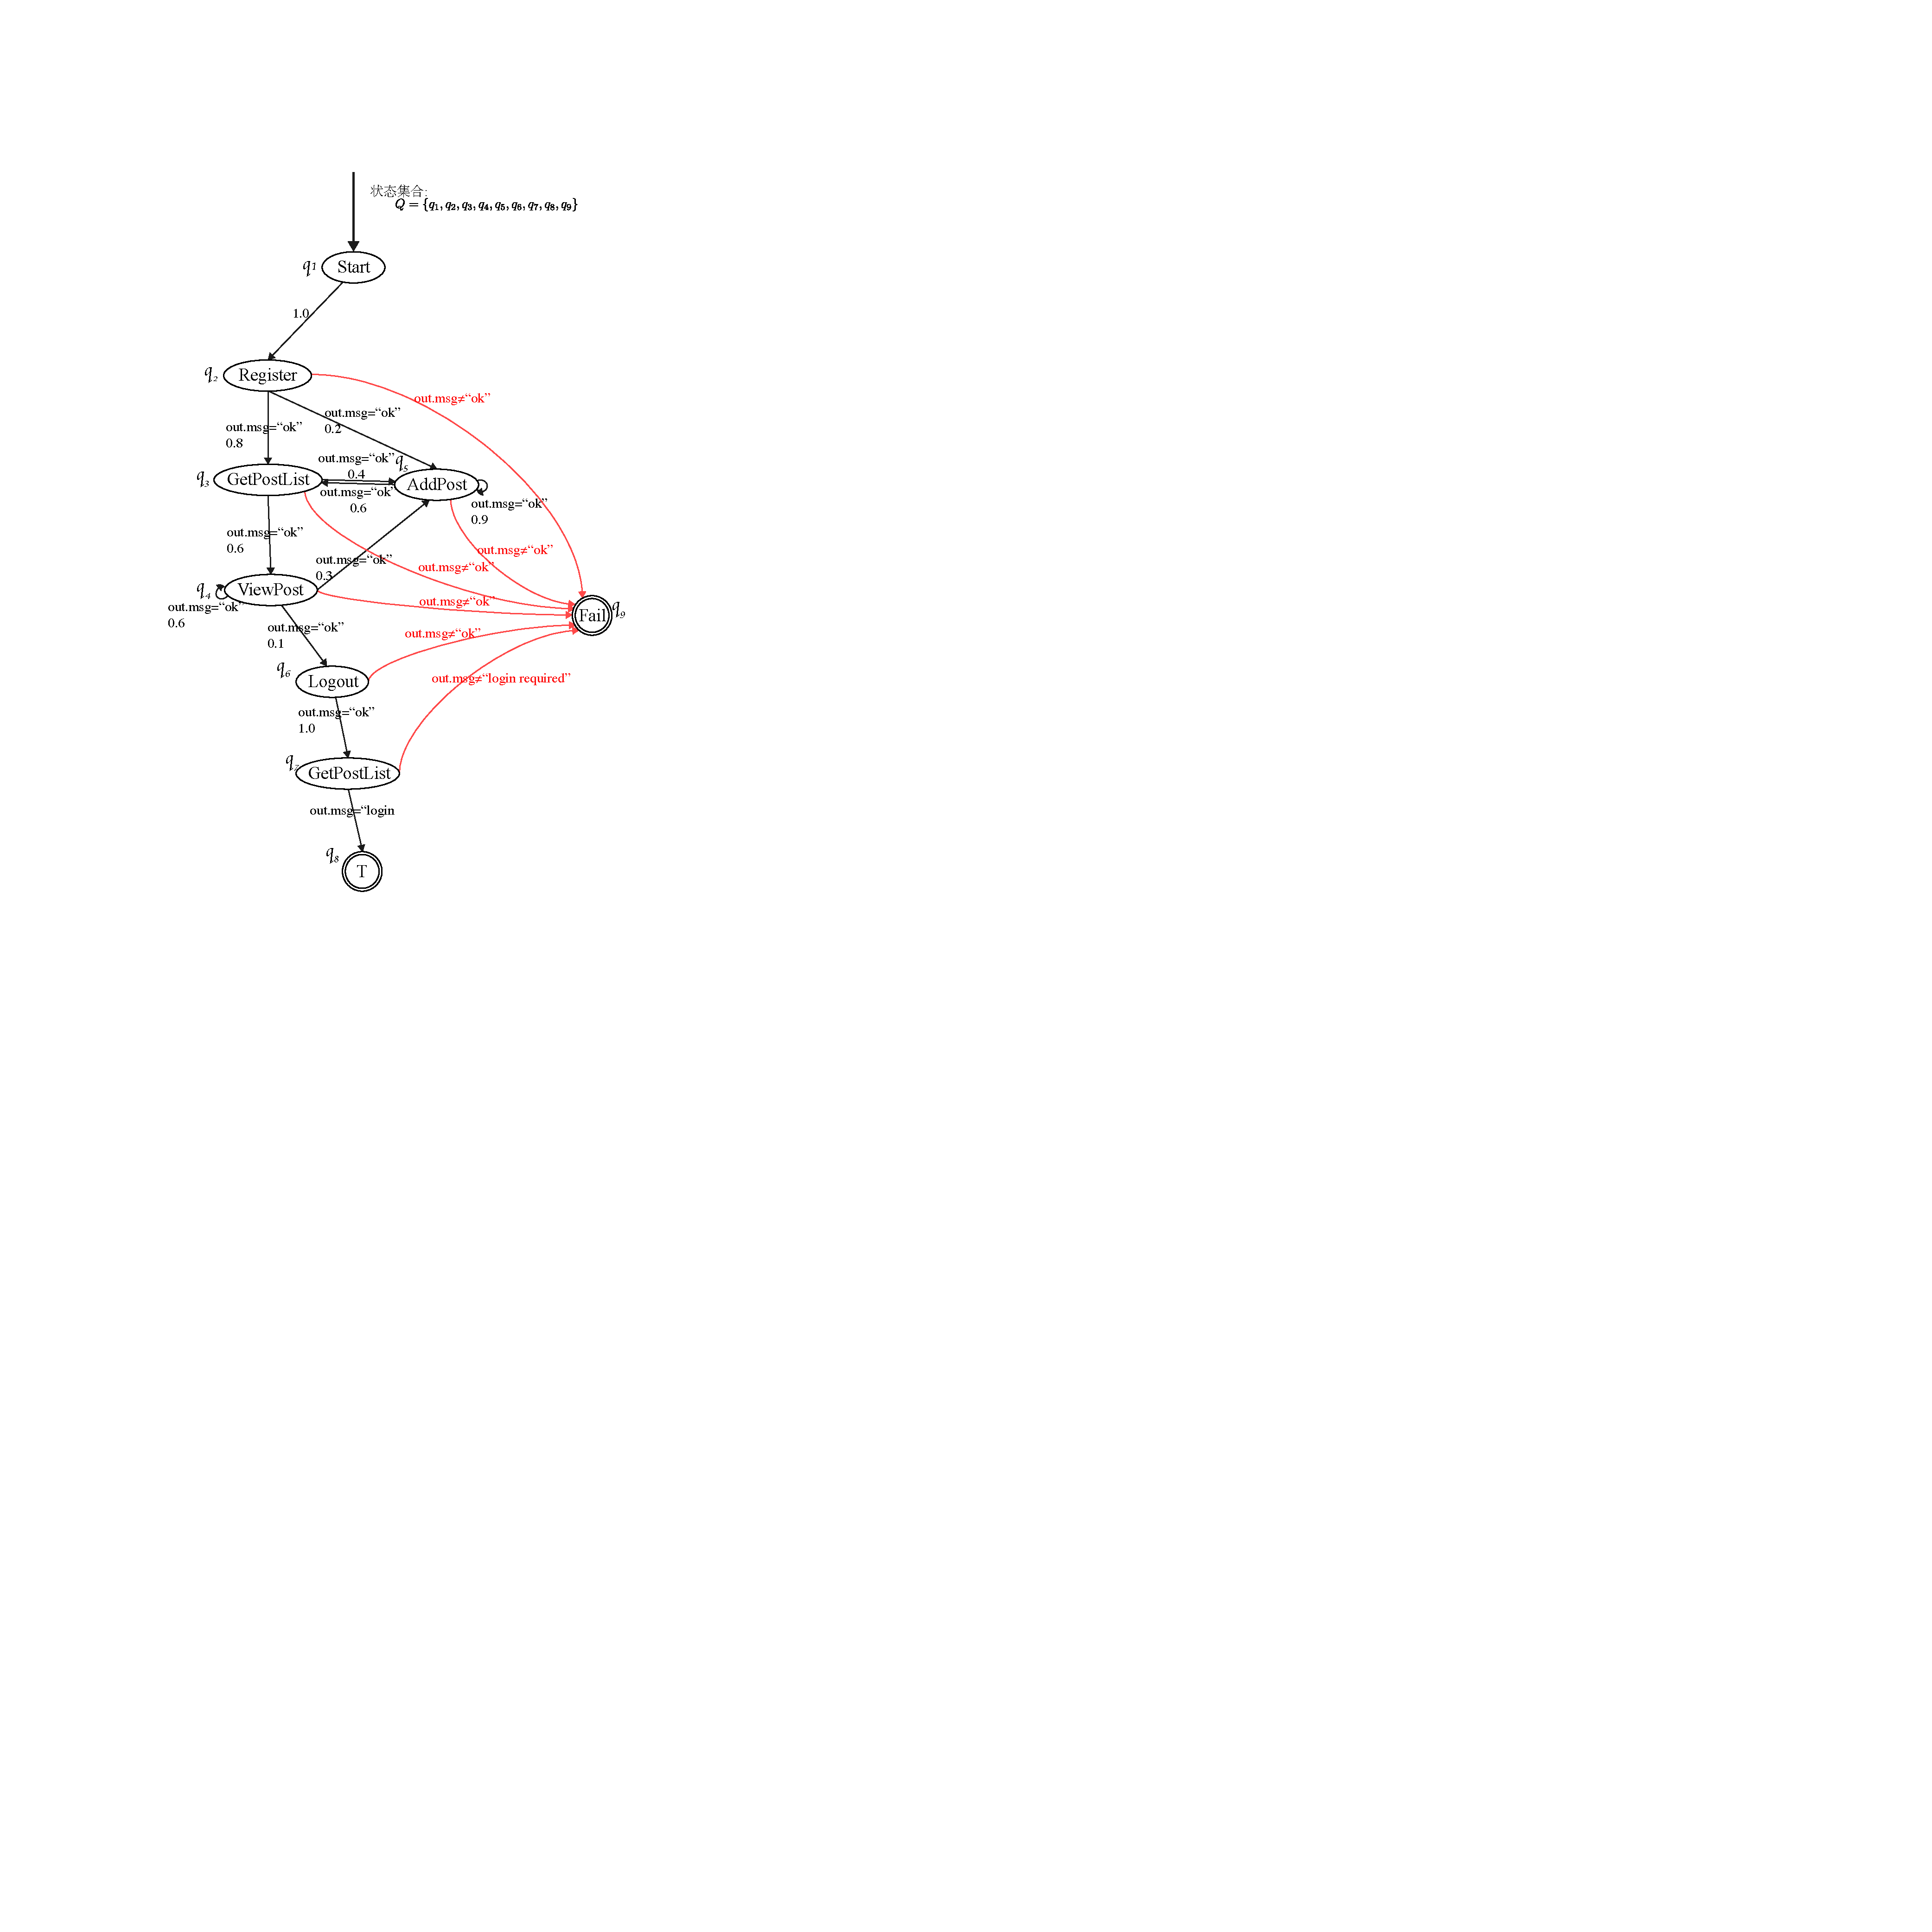
\includegraphics[width=300pt]{scenario_example.pdf}
            \caption{一个场景模型的实例. 请求数据依赖为: \\
            $q_3$.\texttt{request.username} = $q_2$.\texttt{request.username};\\
            $q_3$.\texttt{request.ssid} = $q_2$.\texttt{response.ssid};\\
            $q_4$.\texttt{request.username} = $q_2$.\texttt{request.username};\\
            $q_4$.\texttt{request.postId} = $q_3$.\texttt{response.posts}.\\
            这里, 状态集合的定义($q_d$)和函数的定义($f_d$)以以上谓词形式给出. 起始状态为$q_1$, 终止状态为$q_8, q_9$, 是确定性的.}
            \label{fig:scenario_example}
        \end{figure}
        
        图\ref{fig:scenario_example}为一个典型的场景模型的示例. 这个场景模型是为一个类似微博的自媒体平台服务设计的. 在这个服务里, 用户可以登录, 浏览微博, 发布新微博. 此web服务开放的5个API接口为: “Register”(注册)、“GetPostList”(获取动态)、“ViewPost”(浏览微博)、“AddPost”(发布)、“Logout”(登出). 在图中, 类似自动机模型的表示方法, 使用图的节点来表示场景模型的状态, 节点上的文字表示关联的API或本身含义, 图的边表示场景模型的转移, 边上的数字表示转移概率, 边上的文字表示转移条件.
        
        示例中共有9个状态, 依次从$q_1$编号至$q_9$. 其中$q_1$为确定性的起始状态, 模型工作时状态序列均从$q_1$开始, 该状态未与任何API服务端点关联, 在执行到这一端点时不会发送任何请求. $q_8$("T")和$q_9$("Fail")则为确定性的终止状态, 也就是说, 在其他状态上模型均不会正常终止, 而一旦进入这两个状态, 则必会终止. 其中, 在$q_8$("T")状态结束表示测试通过, 而在$q_9$("Fail")状态结束则表示测试未通过, 该状态亦可通过使式\ref{eq:model_normal2_relax}不取等来隐式定义出来.
        
        示例中共有18项转移, 转移上的表达式, 如\texttt{out.msg} = \texttt{"ok"}和\texttt{out.msg} $\neq$ \texttt{"login required"}, 定义了转移进行的条件, 即, 只有当响应数据\texttt{out}满足条件时, 才可以使用对应转移边. 实际上, 由于转移定义在状态集与响应数据集合的直积上, 而一个表达式条件对应着多个满足条件的响应数据, 故一项表达式表示的条件转移对应着多项实际的转移, 为了简化, 此处均以条件归类表示. 在图中, 正常响应数据的转移使用黑色边表示, 转移条件亦可起到响应数据断言的作用. 异常响应数据的转移则使用红色边表示, 这些边直接指向"Fail"状态, 表示检测到web服务的故障, 测试失败.
        
        部分转移边上存在数字标注, 这些数字表示转移的概率, 各个转移概率不是均等的, 这反映了实际使用场景中不同API的调用频率的不同.
        
        除了图上的部分, 场景还包括请求数据的依赖与响应数据的断言部分, 在此场景示例中, 仅有请求数据的依赖, 响应数据断言则依靠转移条件表达. 这部分在图\ref{fig:scenario_example}的文字部分以谓词表达式的形式具体列出. 如$q_3$\texttt{.request.username} = $q_2$\texttt{.request.username}表达的数据依赖为
        \begin{equation}
            d_{q_3} := <q_2, -1, f(in, out) = \left\{username: in.username;\dots\right\}>.
        \end{equation}
        其含义为, 在$q_3$中, 请求数据的$username$域的值为最近一次到达$q_2$时, 其请求数据的$username$域. 即调用获取动态列表API时, 用户名参数应与之前注册时的用户名相同. 其他各数据依赖项的解读方式类似. 可见, 请求数据依赖信息的加入明显提升了模型表达能力.
        
        此场景模型建模的实际使用场景的含义为: 用户首先进行注册($q_2$, "Register"), 注册时自动登录. 登录后, 用户获取微博的动态列表($q_3$, "GetPostList")或者发布新微博($q_5$, "AddPost"), 用户查看了动态列表之后, 可能浏览某一条具体微博($q_4$, "ViewPost")或者发布新微博. 而在浏览具体微博后, 用户可能继续浏览其他微博(以$q_4$上的自环表示)或者有感而发并发布自己的新微博. 发布完微博后, 用户可能会连续再发布一条刷屏(以$q_5$上的自环表示)或者返回查看动态列表寻找其他动态. 再之后, 可能在浏览到某一条微博后用户感到厌倦, 从而选择登出($q_6$, "Logout"). 为了测试登出的效果, 登出后会试图再次获取微博的动态列表($q_7$, "GetPostList"), 此时应该提示要求重新登录, 若是此提示, 整个测试成功, 一次用户会话亦结束. 可以看出, 场景模型在此示例中较细致地对用户使用web服务的行为进行了建模, 并同时兼顾了API组合测试的需求.
    
    \section{场景模型构建}
        \label{sec:scenario_build}
    
        构建本文中提出的场景模型有着多种方法.
        
        首先, 由于场景模型有着严格的形式化定义, 可以很方便地将之脚本化, 因此便可以使用脚本描述测试场景. 为了基于场景模型进行自动化测试, 我们已经定义了一套基于YAML格式的测试场景描述语言, 如图\ref{fig:scenario_script_eg}即为一段可在本文工具中直接解析与使用的该描述语言编写的场景脚本(有省略), 该场景模型描述了键值对增删服务的一个使用场景, 它的对应有向图表示为图\ref{fig:scenario_script_graph}. 可以看出, 由于模型本身与描述语言的简练性, 简短的脚本便可以描述有一定意义的场景模型.  故人工使用场景描述语言编写脚本的工作量并不大.
        
        \begin{figure}[!htb]
            \centering
            \scriptsize
            \tt
            
            \begin{lstlisting}[language=yaml]
name: InsertTesting
description: Testing large scale element insert and delete operations
nodes:
  -
    name: s
    startWeight: 1.0
    action: {operationRef: 'root#/paths/\/map\/clear/get'}
  -
    name: i
    repeatTime: 16
    action: {operationRef: 'root#/paths/\/map\/insert/get'}
  -
    name: gs
    action: {operationRef: 'root#/paths/\/map\/get_size/get'}
  -
    name: gk
    action: {operationRef: 'root#/paths/\/map\/get_keys/get'}
  -
    name: d
    action:
      operationRef: 'root#/paths/\/map\/delete/get'
      paramConstraint:
        key:
          fromPrevious: {nodeName: gk, seqIndex: -1, rValue: '$response.body#/keys/0'}
  -
    name: e
    endProbability: 1.0
edges: [{from: s, to: i}, {from: i, to: gs}, {from: gs, to: gk},
   {from: gk, to: d, condition: '...'}, {from: d, to: gk},
   {from: gk, to: i, weight: 0.5, condition: '...'},
   {from: gk, to: e, weight: 0.5, condition: '...'}]
            \end{lstlisting}
            
            \caption{键值对增删服务的一段场景脚本(有省略). 此场景描述了该服务的一个完整场景模型.}
            \label{fig:scenario_script_eg}
        \end{figure}
        
        \begin{figure}[!htb]
            \centering
            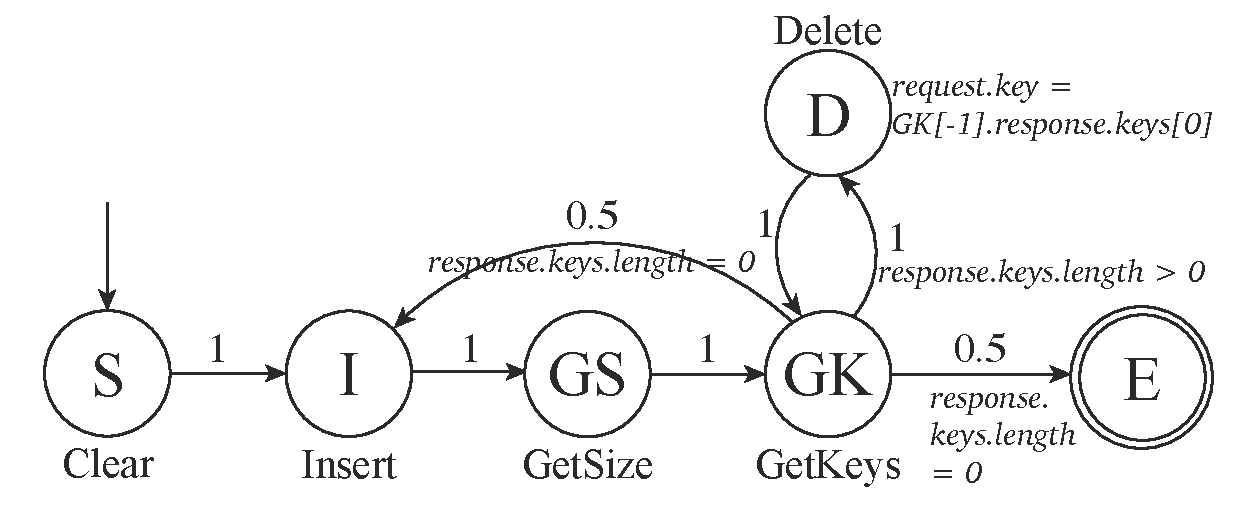
\includegraphics[width=400pt]{scenario_script_graph.pdf}
            \caption{键值对增删服务的场景脚本(图\ref{fig:scenario_script_eg})对应的场景模型.}
            \label{fig:scenario_script_graph}
        \end{figure}
        
        采用绘制与拖拽编辑有向图, 则是更高级方便的场景模型的手工构建方法. 由于场景模型基于自动机模型而扩展, 故类似于自动机, 带有注解的有向图仍是其有效的表示方式. 使用交互式的GUI, 用户可以直接对有向图以拖拽和绘制方式直观地进行编辑, 进一步提高场景模型的设计与构建效率. 目前, 有向图编辑的GUI在web端和桌面端均不难实现, 很多前端库Qunee\footnote{qunee.com}, State.js\footnote{https://github.com/steelbreeze/state.js}均提供了此功能, 本文的LapisGUI编辑工具亦基于PyQt提供了此功能.
        
        场景模型的构建亦可以进行一定程度的自动化. 在描述API的行为与要素的OpenAPI语言中, 存在一个名为\texttt{links}的域用来描述当前API与其他API在设计环节的关联, 这里的关联仅描述后继执行的API. 它不仅可以指定后继API的名称, 还可以指定数据流的依赖和传递关系, 如后继的各请求参数分别如何复用当前API的请求数据或响应数据. 一个API可以指定多个关联. 依靠API脚本中的这类关联元素, 可以非常容易地挖掘出包含数据流依赖的频繁调用序列. 更进一步地, 正如\ref{sec:research_status}小节所述, 在数据挖掘与代码分析领域, \inlinecite{fowkes2016parameter}, \inlinecite{taox06}, \inlinecite{Zhong2009}等工具已经提出了较为完善的API频繁调用序列的自动化挖掘方法. 近年来, 随着基于神经网络的深度学习方法的发展与运用, 从自然语言的文档描述中学习API用法和调用序列成为了一个很具有可行性的学习任务, \inlinecite{xiaodongg16}工作即为一个典型示例, 此学习任务的结果输出也是API的调用序列. 这些使用全自动化方法获得的调用序列均可以有效辅助场景构建, 提高构建场景的效率.
        
        场景模型构建还可以进一步自动化. 在基础算法方面, \inlinecite{anand97}工作在很早之前即提出了从序列分布中学习概率有限状态自动机的快速算法. 由于本文的场景模型即基于此自动机, 进行一定的扩展, 则从调用序列的分布中全自动学习出场景模型也很可能具有可行性. 主要的扩展工作应该在于保证调用序列的完备或处理调用序列不完备的情况, 以及数据依赖, 约束与断言的挖掘与学习. 这是值得进一步讨论的未来研究方向.
        
    \section{对比}
        目前, 对于web API, 亦有其他场景建模与自动化测试法. 本小节将本文提出的场景模型与学术界相关工作、和工业界仍普遍采用的手工脚本模型, 从表达控制流能力、表达数据流能力以及测试用例多样性方面, 进行了简要对比.
    
        具体来说, 考虑以下三种场景模型作为对照:
        \begin{itemize}
            \item 概率转移图\cite{junyiw17}: 此模型使用定义了起始节点和终止节点集合的有向概率图表达使用场景. 在图上进行遍历, 并根据出边的权值概率性地选择下一节点, 重复此过程, 便可以自动化地生成测试用例.
            
            \item 请求序列: 在代码分析和数据挖掘领域, 常使用请求序列对API使用场景建模. 如文献\inlinecite{taox06}\inlinecite{xiaodongg16}中, 就使用代码静态分析和数据挖掘方法, 从开源仓库中获得API请求序列的频繁模式. 这种请求序列可以使用标准化格式编码, 然后导入既有API测试工具进行自动化测试, 如Swagger Inspector\cite{swaggerinspetor17}.
            
            \item 测试脚本: 在工业界, 最常见的测试方式仍然是使用测试人员手工编写的测试脚本. 这里可以将测试脚本视为场景模型的一种描述.
        \end{itemize}
        
        \begin{table}[!htb]
            \centering
            \begin{tabular}{ccccc}
                \toprule
                 & 自动化程度 & 控制流 & 数据流 & 测试用例多样性 \\
                \midrule
                本文的 & 手动/半自动 & 顺序, 循环,  & 数据复用 & 富有 \\
                场景模型   & 构建 & 条件与概率转移 & 数据依赖 & 多样性 \\
                \hline
                \multirow{2}{*}{概率转移图\cite{junyiw17}} & 手动 & 顺序与 & \multirow{2}{*}{无} & 较富有 \\
                & 构建 & 概率转移 &  & 多样性 \\
                \hline
                \multirow{2}{*}{请求序列\cite{taox06}\cite{xiaodongg16}} & 自动 & \multirow{2}{*}{顺序} & 数据复用 & 固定序列, \\
                & 构建 &  & 数据依赖 & 缺少多样性 \\
                \hline
                \multirow{2}{*}{测试脚本} & 手动 & 可完全 & 可完全 & 取决于 \\
                & 构建 & 编程自定义 & 编程自定义 & 具体脚本 \\
                \bottomrule
            \end{tabular}
            \caption{本文场景模型与其他常用测试场景模型的对比.}
            \label{tab:related_work_compare}
        \end{table}
        
        表\ref{tab:related_work_compare}对这些不同场景模型进行了对比. 
        
        在自动化程度方面, 基于本文的场景模型, 自动化测试时只需构建抽象的场景模型即可. 由上文对模型构建的讨论可知, 这种构建过程可以是手动或半自动的, 依靠模型便可自动化生成测试用例. 概率转移图模型与之类似, 但概率转移图需要手动构建. 请求序列模型基于自动化挖掘出的频繁序列模式, 可全自动构建. 而测试脚本则需完全手动编写.
            
        在控制流方面, 本文提出的场景模型支持顺序、循环、条件与概率转移, 能力可与过程式程序语言媲美. 并且, 概率分布函数还对随机性和概率性进行了抽象, 表达简洁清晰. 概率转移图模型仅支持顺序与概率转移, 但也对概率性进行了抽象. 而请求序列模型则仅支持顺序执行. 测试脚本模型基于程序语言, 能力与程序语言的控制流表达能力等价, 不过对概率性的表达较复杂.
            
        在数据流方面, 本文提出的场景模型可描述数据复用与数据依赖, 以及基于数据约束的条件转移, 与程序语言的能力近似. 概率转移图模型不支持数据流描述, 以及条件转移. 请求序列模型如果进行一定的扩展, 则也可以支持数据复用与数据依赖的描述. 而测试脚本基于程序语言, 描述能力与可执行程序相同.
            
        在测试用例多样性方面, 由于在状态序列生成和请求数据生成(见\ref{sec:req_data_gen}小节)中均引入了概率性和随机性, 本文提出的场景模型可自动生成具有相当多样性的测试用例, 并满足多种覆盖率要求. 概率转移图模型由于缺乏数据流表达能力, 生成的测试用例仅具有图上的路径多样性, 但测试数据多样性不足. 请求序列模型只能生成固定执行序列, 测试用例几乎不具有多样性. 测试脚本模型的用例多样性则取决于具体脚本, 但由于概率性与随机性的表达在程序语言中较繁琐, 实际上单个测试脚本生成的测试用例常常不具备太强的用例多样性, 而是依靠脚本的大数量规模来实现.
        
        综合对比以上场景模型, 可以看出各种模型各有优劣. 其中, 本文提出的场景模型的主要劣势在于自动化程度尚有一定不足, 不能全自动构建场景模型. 除此之外, 在测试能力方面则十分理想, 几乎接近自由度最高的测试脚本方法, 且表达更简洁清晰, 相比其他场景模型有明显优势.
    
